Os resultados alcançados no projeto se dividiram em duas fases diferentes: o \textit{software} GPSATWeb, desenvolvido para aplicação da ficha de avaliação dos amputados; a RNA, que apresenta uma análise da condição de pele dos amputados com a utilização de fotos como dados de entrada.

O \textit{software web} foi finalizado e é funcional. Este sistema visa facilitar e agilizar a aplicação e o preenchimento da ficha de avaliação dos pacientes amputados, além de salvar seguramente seus dados e gerar um relatório da avaliação contendo o histórico do paciente.

A RNA trabalhada foi construída em um processo iterativo de variação de entrada para que sua precisão fosse gradualmente aumentada a cada iteração. No início do processo foi construída também uma RNA utilizando outro método de treinamento a título de comparação, o crescimento da precisão da RNA MLP, pode ser visto na Figura 9.

\begin{figure}[ht]
    \centering
    \label{fig09}
        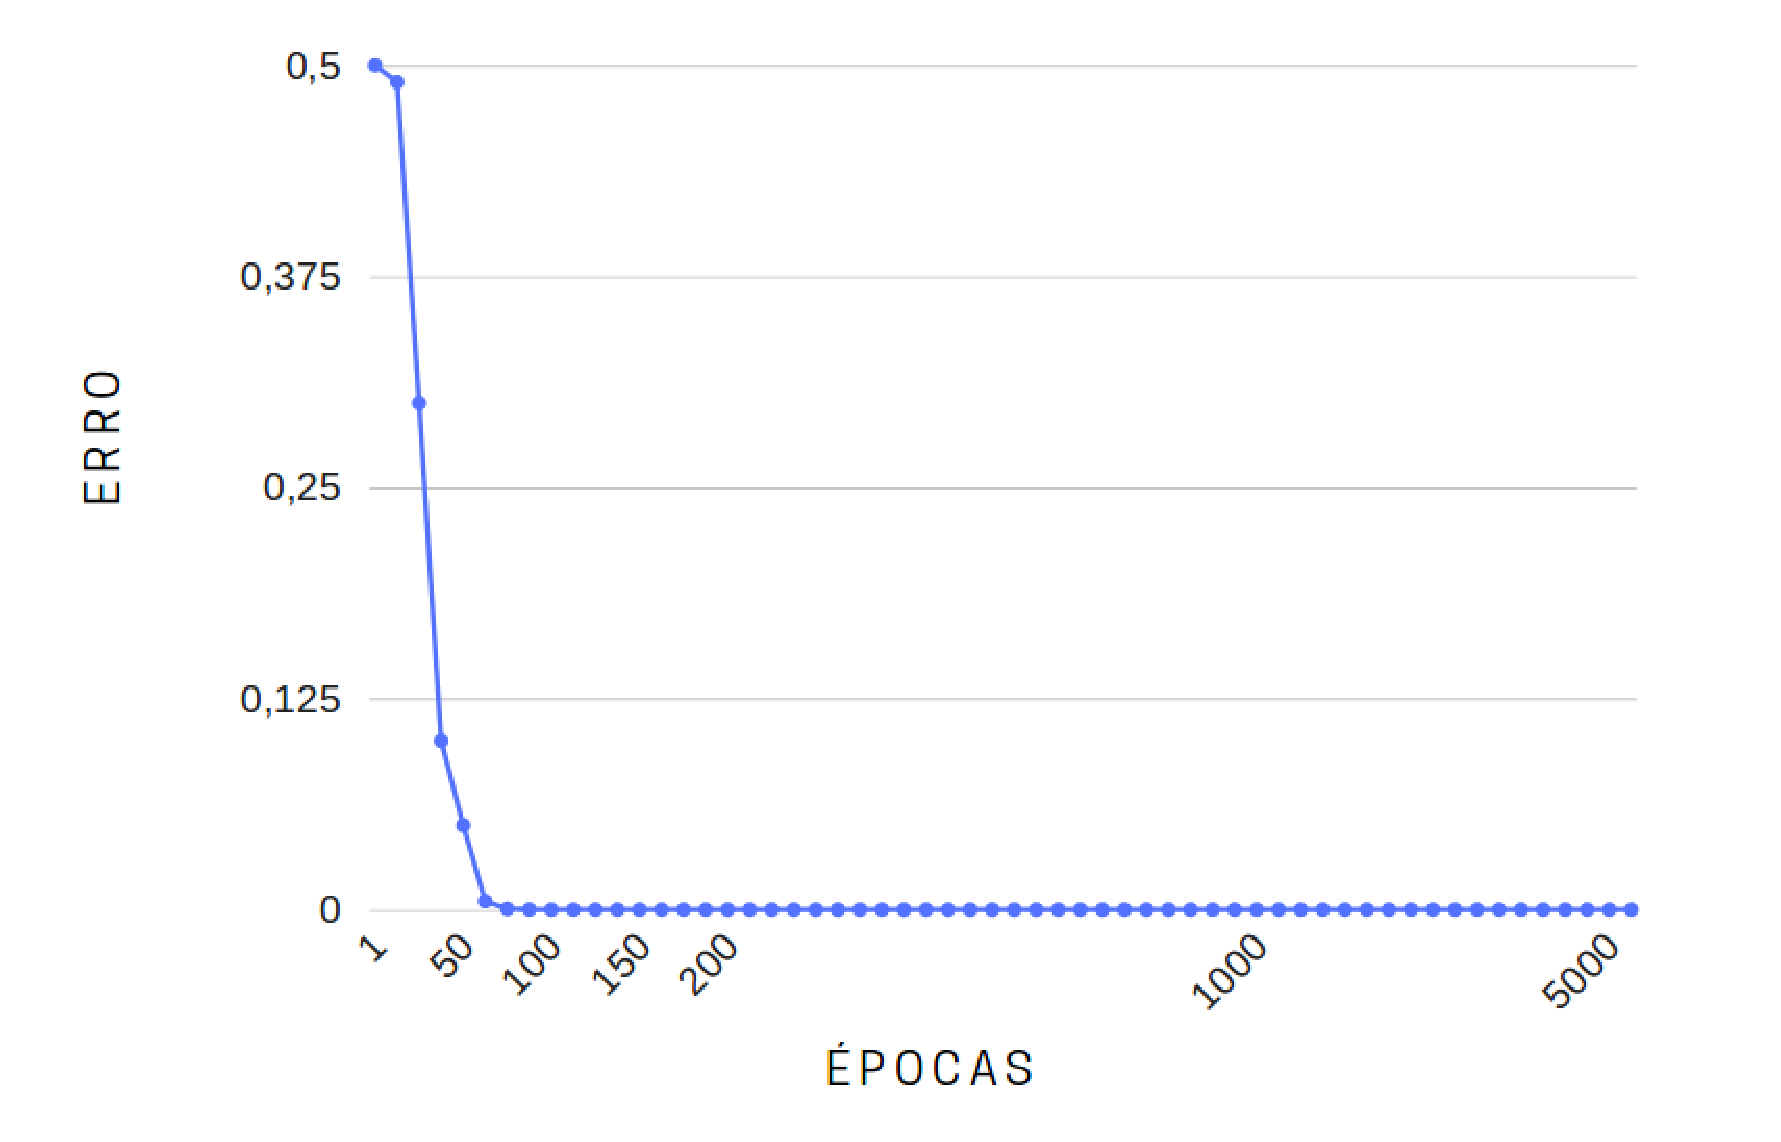
\includegraphics[keepaspectratio=true, scale=0.4]{editaveis/images/grafico_rna.eps}
    \caption{Gráfico de Evolução da RNA}
\end{figure} 

 Como o processo iterativo viria a ser muito longo, foram marcados no gráfico somente os pontos onde ocorreu variação de pelo menos 1\% no valor da precisão da RNA MLP. O salto de produtividade da precisão da RNA MLP se deve à uma decisão de projeto de dividir cada uma das imagens produzidas na sessão de fotos em quadrados de 32x32 \textit{pixels}, aumentando assim a amostra de imagens geradoras de dados para treinamento da RNA, além do início do uso de \textit{bias}.


% - - - - falar sobre IA explicitamente - - - -  \\
% - - - - descrever resultados de rna com estatística - - - -  